\chapter{Results}
\label{ch:results}

\section{Participant descriptions}

\subsection{User participation}

The \nameref{app:participation} appendix on page~\pageref{app:participation} shows statistics on how many days the different used the system. In table~\ref{tab:participation_incl} it is shown that in total 63 students made an account within the system. From these students 44 used the system on at least one day for longer than 15 minutes, of which the average student participated on 4.68 days. These statistics are also summarised within figure~\ref{tab:participation}. The usage of the system is also depicted in figures~\ref{fig:participation} and~\ref{fig:participation_gen}. Finally, figures~\ref{fig:activedays_fc}, \ref{fig:activedays_fm}, and \ref{fig:activedays_gen} within the appendix display on which days users have been actively using the system as a scatter diagram, and how many users cummulatively have finished using the system as a step diagram, for the flashcard and flashmap seperately and the combined conditions, where day 0 is the day the system was introduced within the presentation and day 21 the final day before the exam.

Interesting to note here is that there are two subsequent strong increases in finished users around 6 days after the system was introduced, but that there is also a very strong increase the day before the students' exam. This is also reflected within a highly increased activity within the first week, and on the day before the exam. There is even some noticable activity after the exam took place, possibly of students already having invested some time into the system before the exam, but still finishing up in order to be rewarded with the icecream voucher. This resulted in a total number of 25 finished users, of which 13 users within the flashcard condition and 12 users within the flashmap condition. Both in the flashcard and the flashmap condition there is one user which did use the software for 6 days, but then did not partake in the posttest.

Within the interviews, it was gathered that students were mainly interested in participation because they had problems preparing the previous exams from the same course and that they believed the system to help them being better prepared. The icecream voucher was only a secondary motivator, but was indicated to be a motivator for persistent use of the software. One student indicated that the system might however be more successful within younger students, since the older students often already have their own learning systems and prefer to stick to these systems.

A sample of 23 divided over two conditions is too small for making any generalisations, and therefore any results stemming from this experiments are only indicatory and should be further investigated before they can be used. Since the only students usable for the rest of the result section are those finishing the posttest, the other students will be omitted from consideration.

\begin{table}
    \centering
    \begin{tabular}{lrrrrr}
        \toprule
        & $\mu_{fc}$ & $\mu_{fm}$ & $p$ \\
        \midrule
        Including zero days & 3.27 & 3.27 & 0.994 \\
        Excluding zero days & 4.32 & 5.16 & 0.984 \\
        \bottomrule
    \end{tabular}
    \caption{Compact view of the participation statistics for both all enrolled users and only including the users with at least one day of participation}
    \label{tab:participation}
\end{table}

\begin{figure}
    \centering
    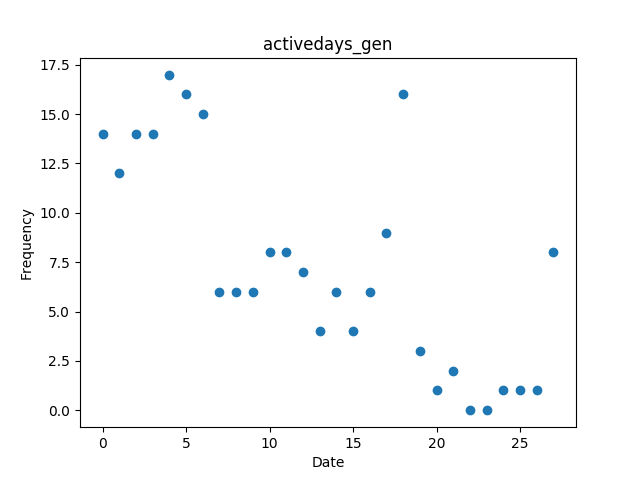
\includegraphics[width=.7\textwidth]{img/activedays_gen.png}
    \caption{A scatter diagram depicting how many users in total were active during which day of the experiment, combined with a step diagram depicting how many users finished the experiment that day (more than or equal to 6 successful days)}
    \label{fig:activedays_gen}
\end{figure}

\subsection{Descriptive variables}

The participant descriptives are included in the \nameref{app:descriptives} appendix on page~\ref{app:descriptives}, containing distributions of student gender and age.

\paragraph{Gender} As can be seen in figure~\ref{tab:gender}, 15 out of the 23 total participants are male and 8 are female, where within the flashcards condition there is a 7 to 5 ratio and within the flashmap a 8 to 3 ratio. This is probably just coincidental due to the small sample size.

\paragraph{Age} All students have an age within the range of 15 to 17 with an average age of 15.75 and a modus of 16, which is to be expected from VWO4 students. There is also no considerable age difference among the conditions, indicated in table~\ref{tab:age_comp} and figure~\ref{fig:age}.

\begin{table}
    \centering
\begin{tabular}{lrrrr}
\toprule\addlinespace
& Total & Male & Female & Other
\\\addlinespace
\midrule
\textbf{Flashcards} & 12 & 7 & 5 & 0
\\\addlinespace
\textbf{Flashmap} & 11 & 8 & 3 & 0
\\\addlinespace
\textbf{Total} & 23 & 15 & 8 & 0
\\\addlinespace
\bottomrule
\end{tabular}
\caption{The gender distribution of the respondents}
\label{tab:gender}
\end{table}

\begin{table}
\centering
\begin{tabular}{lrrrrrrrrrr}
\toprule\addlinespace
& N & min & max & mean & var & skew & kurt & normal-t & normal-p
\\\addlinespace
\midrule
\textbf{Flashcards} & 12 & 15 & 17 & 15.75 & 0.39 & 0.15 & -0.52 & 0.096
& 0.9530
\\\addlinespace
\textbf{Flashmap} & 11 & 15 & 17 & 15.73 & 0.42 & 0.25 & -0.62 & 0.211 &
0.8997
\\\addlinespace
\textbf{General} & 23 & 15 & 17 & 15.74 & 0.38 & 0.20 & -0.57 & 0.307 &
0.8576
\\\addlinespace
\bottomrule
\end{tabular}
    \caption{The age distribution of the respondents}
    \label{tab:age}
\end{table}

\section{Learning gain}

The pre- and posttest statistics are displayed in the \nameref{app:learning_gain} appendix on page~\ref{app:learning_gain}, divided in the inter-rater reliablity statistics and the result scores on the test. 

The results are separately described for the knowledge questions and comprehension scores on the test, since they measure different variables. The different scores described and compared are the pretest scores, posttest scores, total scores, and the absolute (abs) and relative learning gains (rel). Additionally, they are reported as classical test theory scores (ctt), item response theory person abilities (irt), and person abilities from item response theory using fixed item difficulties from the combined pretest scores (fixed irt). Per category, the sample size, minimum, maximum, and mean values are displayed as descriptive values; the skew, kurtosis, and t and p values from the scipy normaltest are displayed as values for describing the distribution of the results; and $\alpha$ describes the reliability of the test (either Cronbach's alpha for the ctt results or the EAP value for the irt results). These results are described for the flashcard condition, the flashmap condition, and the combined sample of both conditions. The included graphs display histograms depicting the test matrices. Finally, the pre- and posttest scores are compared with each other by means of the non-parametric Mann-Whitney U test and the parametric Welchs' t-test in order to verify that users scored significantly higher on the posttest than on the pretest, and the learning gains between conditions are compared in order to answer research question~\ref{benefit}\ref{effectiveness}.

Remarkable are the low scores on the tests, with on average only 1.3 points on the knowledge questions (0.43 on the pretest and 2.17 on the posttest) and only 1.33 points on the comprehension questions (0.33 on the pretest and 2.33 on the posttest). This would indicate that the tests are exceptionally difficult, even though the questions are directly derived from the textbook itself and the users drilling these questions over the course of 6 days. Especially the low posttest knowledge question scores from the flashcard group are striking, since these questions were literally rehearsed during the experiment.

For both the knowledge questions as for the comprehension questions, the ctt reliability for the combined pre- and posttest score for the combined flashcard and flashmap users is around .7 --- mainly because the omission process of unreliable items ---, whereas the fixed irt reliability is around .6 (see table~\ref{tab:know_gen} and table~\ref{tab:comp_gen}). According to \citeA{devellis}, this means that the results obtained from classical testing are acceptable, whereas the results obtained from the item response theory are questionnable at best. Additionally, both the score outcomes, the figures, and the pre- and posttest comparisons in tables~\ref{tab:know_pp_fc_comp}, \ref{tab:know_pp_fm_comp}, \ref{tab:know_pp_gen_comp}, and tables~\ref{tab:comp_pp_fc_comp}, \ref{tab:comp_pp_fm_comp}, \ref{tab:comp_pp_gen_comp} indicate an average positive learning gain from the classical test theory, but a negative gain from the item response theory. Therefore, the conclusion will be based on the results from the classical test theory only.

Table~\ref{tab:learning_gain_effect} summarises the results related to learning gains. In the rows, the absolute and the relative classical test scores and the absolute item response theory person ability scores with fixed item difficulties are included for both the knowledge and comprehension questions. The item response theory results are only included for reference, and from this only the absolute learning gains are taken into consideration, since the person abilities are already estimated relative to the item difficulties. the columns include the reliability, the p-value of the normality test, the flashcard and flashmap mean score, and the p-values for in this case the Mann-Whitnney U test, since none of the results seem to be normaly distributed.

The flashmap users seem to have a higher learning gain than the flashcard users on the knowledge questions, and that looking at only the ctt results they seem to have a lower gain on the comprehension questions. None of the Mann-Whitney U test p-values for the ctt results seem to be significant however, so no conclusions can be drawn yet. This is highly likely due to the low response rate, and more significant results might be found when using a larger sample, especially since the difference in mean values are relatively high in comparison to the variance in scores.

\begin{table}
    \centering
    \begin{tabular}{lrrrrr}
        \toprule
        & $\alpha$ & $\mu_{fc}$ & $\mu_{fm}$ & $p$ \\
        \midrule
        \emph{Knowledge} &&&& \\
        \midrule
        abs-ctt & .721 & 1.25 & 2.27 & .394 \\
        rel-ctt & .721 & 0.04 & 0.05 & .464 \\
        irt & .671 & -2.67 & 3.17 & .000 \\
        \midrule
        \emph{Comprehension} &&&& \\
        \midrule
        abs-ctt & .714 & 2.00 & 0.91 & .218 \\
        rel-ctt & .714 & 0.07 & 0.04 & .245\\
        irt & .606 & -1.28 & -.97 & .688 \\
        \bottomrule
    \end{tabular}
    \caption{Compact view of the results relevant for answering research question~\protect\ref{benefit}\protect\ref{effectiveness}}
    \label{tab:learning_gain_effect}
\end{table}

\begin{figure}
    \centering
    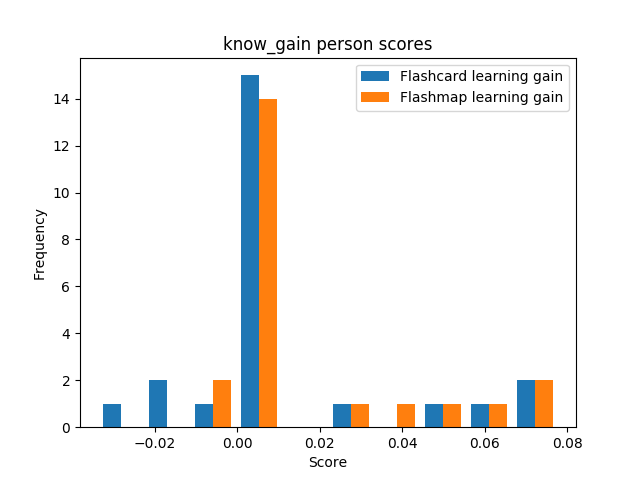
\includegraphics[width=.7\textwidth]{img/know_gain_abil.png}
    \caption{A histogram comparing the relative learning gain scores of the knowledge questions between the conditions}
    \label{fig:know_gain_abil}
\end{figure}
\begin{figure}
    \centering
    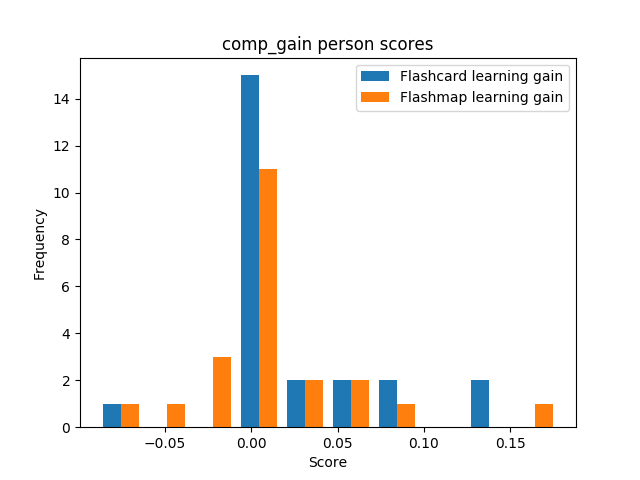
\includegraphics[width=.7\textwidth]{img/comp_gain_abil.png}
    \caption{A histogram comparing the relative learning gain scores of the comprehension questions between the conditions}
    \label{fig:comp_gain_abil}
\end{figure}
\section{System use}

In order to verify whether the users of the different conditions spent the same amount of effort and time on the system, answering research question~\ref{benefit}\ref{efficiency}, the \nameref{app:instance_stats} appendix on page~\pageref{app:instance_stats} provides different statistics on the rehearsed instances. This entails the number of reviewed instances, the number of responses, the exponent from the instance.get\_exponent() function (indicating how often the instance was retrieved correctly since the last incorrect retrieval), the percentage of correct retrievals in comparison to the total amount of retrievals, and finally the amount of time the users spent on the system. For every category, the descriptives (sample, minimum, maximum, mean, and variance), distribution (skew, kurtosis and normality test t- and p-values), and cronbach's alpha are displayed, both separate for the flashcard and flashmap condition and for the combined sample of users. It should be noted that in most cases the cronbach's alpha is not a sufficient measure for determining the reliability of the test, since there is a natural decrease in most statistics over the course of the instances, since the latter instances are repeated less often than the earlier statistics. The ratio of correct retrievals might be the only exception here, however one would still expect a higher ratio of correct retrievals in earlier instances than in later instances. 

Furthermore, the absolute score, the relative score and the mean score are displayed for each condition, where the relative score is the absolute score divided by the total amount of either flashcards or flashmaps. In the combined condition, the relative score is omitted, since the relative score is only useful for comparing the conditions. 

Finally, the flashcard and flashmap conditions are again compared using the Mann-Whitney U test and Welch's t-test. Table~\ref{tab:efficiency} displays all results in a more compact manner.

\begin{table}
    \centering
    \begin{tabular}{lrrrrr}
        \toprule
        & $\alpha$ & $\mu_{fc}$ & $\mu_{fm}$ & $p$ \\
        \midrule
        \emph{Reviewed instances} &&&& \\
        \midrule
        abs & 0.979 & 72.83 & 131.45 & 0.001 \\
        rel & 0.979 & 0.78 & 0.66 & 0.188 \\
        \midrule
        \emph{Responses} &&&& \\
        \midrule
        mean & 0.938 & 7.61 & 5.61 & 0.024 \\
        \midrule
        \multicolumn{5}{l}{\emph{Exponents}} \\
        \midrule
        mean & 0.893 & 6.67 & 6.38 & 0.625 \\
        \midrule
        \emph{Correct retrievals} &&&& \\
        \midrule
        mean & 0.978 & 0.86 & 0.89 & 0.000 \\
        \midrule
        \emph{Time spent} &&&& \\
        \midrule
        abs & 0.924 & 12374.41 & 14121.58 & 0.000 \\
        mean & 0.924 & 169.77 & 117.30 & 0.000 \\
        \bottomrule
    \end{tabular}
    \caption{Compact view of the results relevant for answering research question~\protect\ref{benefit}\protect\ref{efficiency}}
    \label{tab:efficiency}
\end{table}

\paragraph{Number of reviewed instances} Within these statistics, the mean statistics are left out, since they only make sense when reviewing them over the entire range of available instances. Furthermore, the flashcards cannot simply be compared one on one with the flashmaps, since some of the flashcards encompass multiple flashmaps instead of merely representing one flashmaps. This is most notably the case when multiple sibling relations between concepts are presented simultaniously to the user, which are thereby also represented by only one flashcard. Therefore, the combined conditions table only shows the relative score, since this is the only score comparable across both conditions. This is also noticable in the large difference in absolute mean values of the flashcard and flashmap condition (72.83 vs 131.45) and the low p-value on the Mann-Whitney U test (0.001). When however purely looking at the relative score, the average user reviewed 70\% of the available cards, where the flashcard users reviewed 78\% of the cards and the flashmap users 66\%. This difference is not yet significant ($p=.188$ on the Mann-Whiney U test). As can be seen in figure~\ref{fig:instance_abil} on page~\pageref{fig:instance_abil}, this difference is mainly due to both groups having reviewed about equal numbers of instances except for 2 users in the flashmap condition having reviewed less than 50\% of the edges.

\begin{figure}
    \centering
    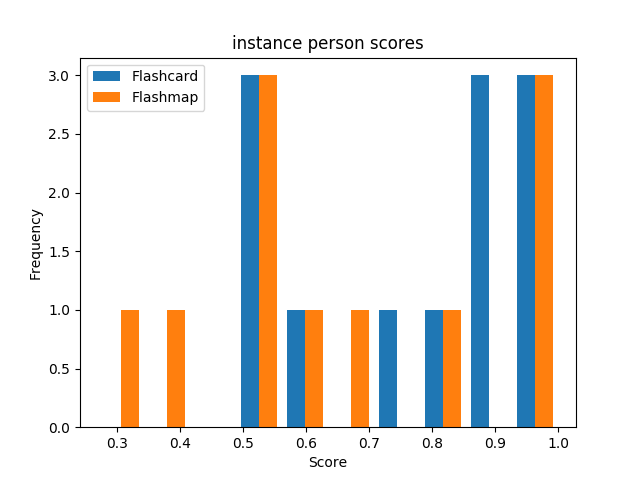
\includegraphics[width=.7\textwidth]{img/instance_abil.png}
    \caption{A histogram depicting the number of instances covered by a user separate for the groups of flashcard and flashmap users}
    \label{fig:instance_abil}
\end{figure}

\paragraph{Number of responses} These first statistics depict the total number of reviews of instances per user. On average, a user has 641.87 responses, where flashcard users have 561.33 and flashmap users have 729.73 responses. Both the Mann-Whitney U test as the Welch's t-test provide a relatively high p-value (.813 and .810) when looking at the difference in relative score, indicating no (significant) difference between the number of responses within the flashcard users and the flashmap users when adjusting for the different numbers of flashcards and edges.

\begin{figure}
    \centering
    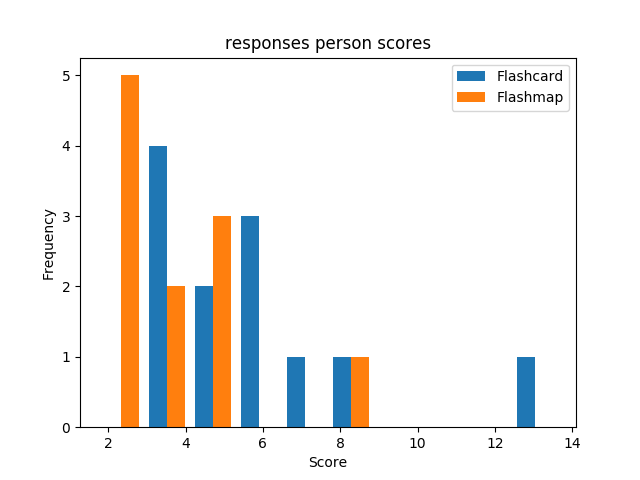
\includegraphics[width=.7\textwidth]{img/responses_abil.png}
    \caption{A histogram depicting the number of responses per user separate for the groups of flashcard and flashmap users}
    \label{fig:responses_abil}
\end{figure}

\paragraph{Exponents} These statistics are useful as an indicator of learning progress of the user, since the exponents are used for rescheduling the instance where a higher exponent indicates a longer time interval until the next review. The mean exponent for a reviewed instance was 6.53, where it was 6.67 for flashcard users and 6.38 for flashmap users. This difference is not significant ($p=0.625$).

\begin{figure}
    \centering
    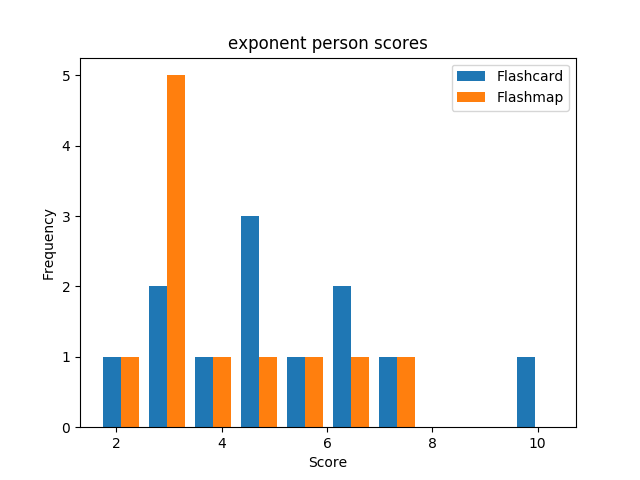
\includegraphics[width=.7\textwidth]{img/exponent_abil.png}
    \caption{A histogram depicting the exponents per user separate for the flashcard and flashmap users}
    \label{fig:exponent_abil}
\end{figure}

\paragraph{Correct retrievals} The ratio of correct and total retrievals is also included, since this provides more insight in the effectiveness of the scheduling algorithm and the presentation form. For each reviewed instance, the ratio of correct and total retrievals is 0.87, where 0.86 for flashcard and 0.89 for flashmap users. This results in a small although significant ($p<0.001$) difference in favour of the flashmap users. In the interviews however some students stated to not have noticed the instructions teaching how to mark retrievals to be either correct or incorrect, resulting in a 100\% correct retrieval rate within the database (see also figure~\ref{fig:score_abil} on page~\pageref{fig:score_abil}).

\begin{figure}
    \centering
    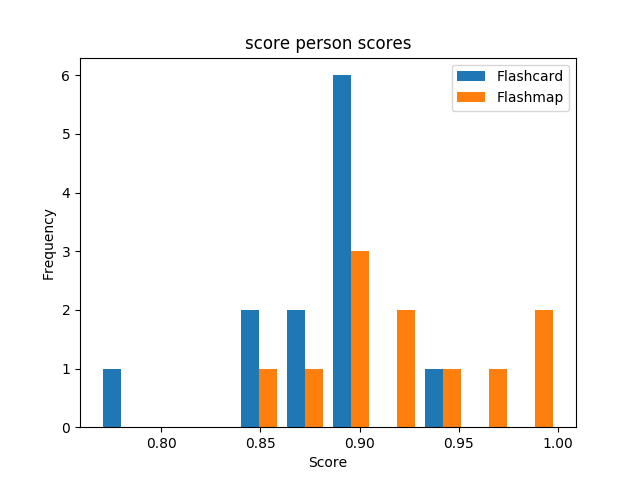
\includegraphics[width=.7\textwidth]{img/score_abil.png}
    \caption{A histogram depicting percentages of correct answers per user separate for the flashcard and flashmap users}
    \label{fig:score_abil}
\end{figure}

\paragraph{Time spent} The most efficient variable for determining the efficiency of the system is the amount of time spent by the user on the system. In total, the average user spent 13210 seconds (3 hours and 40 minutes) on the system, where the average flashcard user spent 12374 seconds (3 hours and 26 minutes) and the average flashmap user spent 14122 seconds (3 hours and 55 minutes). Per instance, this was on average 144.7 seconds, where 169.8 seconds for flashcard users and 117.3 seconds for flashmap users. Both these differences are significant ($p<0.001$).

\begin{figure}
    \centering
    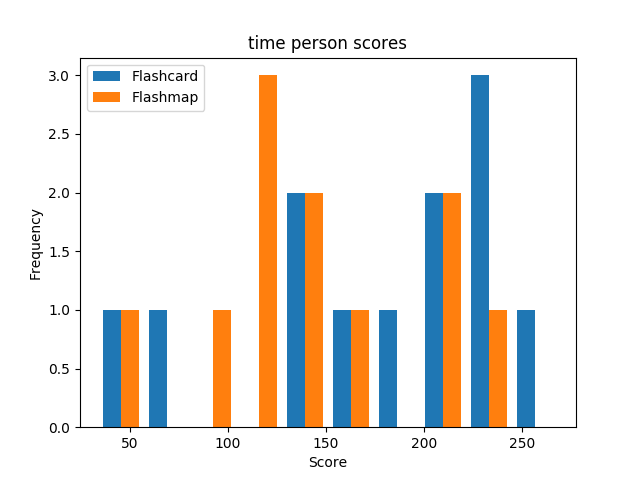
\includegraphics[width=.7\textwidth]{img/time_abil.png}
    \caption{A histogram depicting the time spent in seconds per user separate for the flashcard and flashmap users}
    \label{fig:time_abil}
\end{figure}

\paragraph{Interviews} During the interviews it was learned that the students thought that some of the instances were reviewed too often, sometimes leading to frustration. Some of the students offered the suggestion to add a third validation for a longer scheduling interval, much like Anki already does. Others suggested an option to learn flashcards per section of the instructional material seperately instead of reviewing all the flashcards, so that they could focus on the lesser known or more important sections. Finally, one flashcard user stated that it was not necessary to read the instructional material at all for using the system, and that he learned the flashcards without reading. Other flashmap students however indicated that the book was necessary to comprehend the relations between the concepts.

\section{User perceptions about the software}

Both the question of how useful (research question~\ref{perception}\ref{usefulness}) as of how easy to use (research question~\ref{perception}\ref{ease}) the system is perceived to be is investigated quantitatively as qualitatively by means of the questionnaire, and open questions and the interviews. The quantitative results for both perceived usefulness as perceived ease of use are displayed in table~\ref{tab:perception}.

\begin{table}
    \centering
    \begin{tabular}{lrrrrr}
        \toprule
        & $\alpha$ & $\mu_{fc}$ & $\mu_{fm}$ & $p$ \\
        \midrule
        Usefulness & 0.651 & 6.50 & 8.82 & 0.245 \\
        Ease of use & 0.829 & 6.58 & 8.27 & 0.482 \\
        \bottomrule
    \end{tabular}
    \caption{Compact view of the results relevant for answering research question~\protect\ref{perception}}
    \label{tab:perception}
\end{table}

\subsection{Perceived usefulness}

\paragraph{Questionnaire} The perceived usefulness part of the questionnaire has a relatively low reliability ($\alpha=0.651$), which makes drawing definite conclusions questionable according to \citeA{devellis}. The average perceived usefulness score was 7.61 on a scale of -24 to 24, which indicates a slight positive score. The average flashcard user rated it as 6.50, and the average flashmap user as 8.82. These differences are however not significant ($p=0.245$).

\begin{figure}
    \centering
    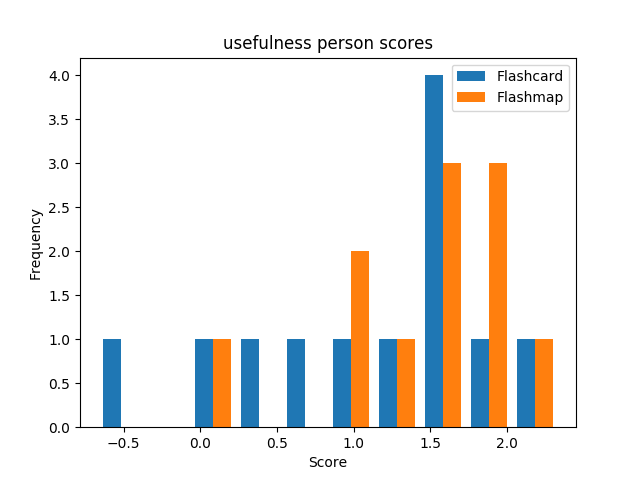
\includegraphics[width=.7\textwidth]{img/usefulness_abil.png}
    \caption{A histogram depicting a comparison of perceived usefulness between the conditions}
    \label{fig:usefulness_abil}
\end{figure}

\paragraph{Open questions} Within the open question asking what the user perceived to be good about the system, students mainly mentioned why the system helped them preparing for the exam. The responses could be categorised in 3 subcategories:
%
\begin{itemize}
    \item the structure provided by the questions
    \item the distribution of learning over a period of time
    \item the repetition of questions
\end{itemize}
%
The first category contains statements about the questions hinting at the important aspects of the text (``It indicates the things that are important'') and about the system providing a certain overview (``It was effective for learning the sequence of the history''). Statements such as ``One learns a small portion every day instead of everything on one day'' were placed in the second category. Finally, the third category contained statements such as ``The repetition, which made the subject matter really sink in'' or ``The incorrect items were repeated so that these answers were learned better''. However, the open question about what could be improved also contained certain comments about the repetition, mainly that certain questions were sometimes repeated too often. One comment also indicated that the questions were rather superficial. Next to these statements, some general comments were made such as ``It was fun to do'' or ``It was convenient''.

\paragraph{Interviews} Within the interview, both flashcard and flashmap indicated that they thought of the tool itself as generally useful for learning textual material, aligning with the questionaire result. Respondents indicated the instances to be easier to comprehend than the textbook itself, and that they performed better on the final test than they normally did. When asked whether they would use a flashcard system again for another subject, they stated that they would definitely do this for other courses based on long texts such as history, but also for subjects like chemistry. One respondent even already used the flashcard system for music history, using the traditional system where every wrong card is rescheduled for today and all other cards are scheduled for the next day. They were also interested in hearing about alternative flashcard systems such as Anki. The flashmap users also stated that they liked the overview of the relations among concepts the map provided, however that this could also be a drawback since the user does not have to draw any connection for himself. The flashcards also did indicate that finding the relations between the concepts in the flashcards was not very difficult.

There were however some problems with the specific implementation. As already stated before, users thought that the instances were reviewed too often, resulting in a too high emphasis on the earlier instances. Furthermore, they did state that the system did not prepare them enough for the final test, mentioning the concept of "petrarkism" as an example. This concept was however present in both the flashcards as in the flashmap, but might have had a too low exposure. Finally, they stated that making the network or flashcards could be beneficiary, because then the relations or questions are better understood instead of only rehearsed.

\subsection{Perceived ease of use}

\paragraph{Questionnaire} The perceived ease of use part of the questionnaire had a sufficiently high reliability ($\alpha=0.829$), and is therefore reliable to be used for drawing conclusions. The average score for the perceived ease of use section was 7.39, which translates again to a slightly positive score. The difference between the flashcard and flashmap users is relatively small (6.58 for flashcard users and 8.27 for flashmap users), which is not significant ($p=0.485$).

\begin{figure}
    \centering
    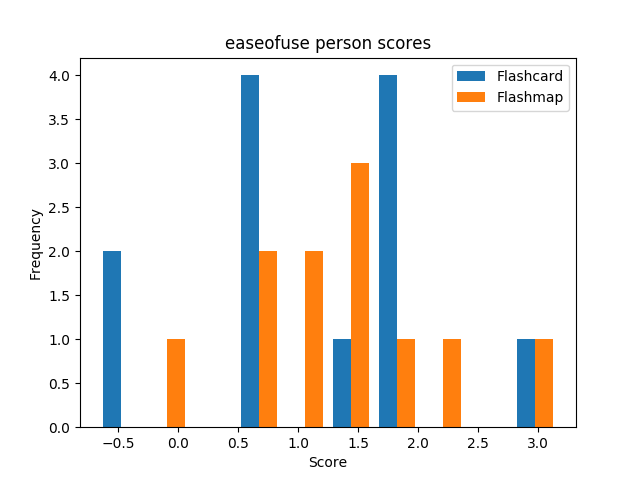
\includegraphics[width=.7\textwidth]{img/easeofuse_abil.png}
    \caption{A histogram depicting a comparison of perceived ease of use between the conditions}
    \label{fig:easeofuse_abil}
\end{figure}

\paragraph{Open questions} Most of the statements about what could be improved related to the ease of use of the system. Some flashmap users stated that certain flashmaps were too large and therefore unreadable, whereas others perceived zooming in and out on the flashmap to be inconveniant. One of the flashcard users indicated that the questions were sometimes unclearly formulated. Some of the users generally stated the instructions should be more clear, or that the indicators could be improved (e.g. ``It was unclear how much one should learn on a day''). Finally, certain students perceived the system to be a bit boring because of the repetitive nature of drill and practice.

\paragraph{Interviews} Within the interviews, the students stated that the system was generally easy to use, again aligning with the questionnaire results. One user however stated that the mobile version of the flashmap system was somewhat less user-friendly, since one had to zoom in and out in order to be able to read the larger concept maps on a smaller screen, and that users had to scroll down to show the answer to the instances. Some of the users did not even know that the flashmap was interactable. For flashcards this was not an issue. Users did agree generally that the instruction panel was quite unclear, either because the instructions were rather sparse, or because the users did not notice the panel or the text changing within the panel. This for example also resulted in users not indicating whether answers were retrieved correctly. They suggested a better introduction at the beginning of the use of the system. Furthermore, the learning progress overview was indicated to be either not very clear in the case of the flashcard system, or not very insightful in case of the flashmap system. Additionally, students mentioned the inconsisency in the graph layout, and that it was not always clear when they were finished for today with regards to the reward. Finally, forgetting to daily use the system was an issue for users, but also the fact that they had to use it daily was conceived as rather rigid.
